\subsection{Motor modelling}
A model of a motor consist of both a mechanical and an electrical system, due to the fact, that electrical current, \si{i_a(t)}, is converted into a rotational force called torque, \si{\tau_m}. A model of the mechanical and the electrical system is therefore created. The mechanical model from the motor provides the contributions the motor delivers to the drivetrain, see \secref{DriveTrain}, and the electrical model provides the motors produced torque.

\subsubsection{Mechanical model}
A mechanical model is formed to analyse the forces and inertias affecting the mechanical system, and to see how the system will react to stimuli.

Newtons second law of motion for rotational systems yields:

\begin{flalign}\eq{
\tau_m(t)} {J_m \cdot \ddot{\theta}_m(t)} \unit{N\cdot m}
\label{eq:mechanicalmodel}
\end{flalign}
\hspace{6mm} Where:\\
\begin{tabular}{p{1cm}ll}
& \si{J_m} & is the motors inertia \unit{kg\cdot m^2} \\
& \si{\ddot{\theta}_m} & is the angular acceleration in the motor \unit{\frac{rad}{s^2}} \\
\end{tabular}

This law is applied to the mechanical model and visualized in \figref{fig:MotorMechanicalModel}. Furthermore it is necessary to consider the friction affecting the rotation of the motor when it is spinning. The friction is in the opposite direction of the applied rotational force torque, see \figref{fig:MotorMechanicalModel}.

\begin{figure}[H]
	\centering
	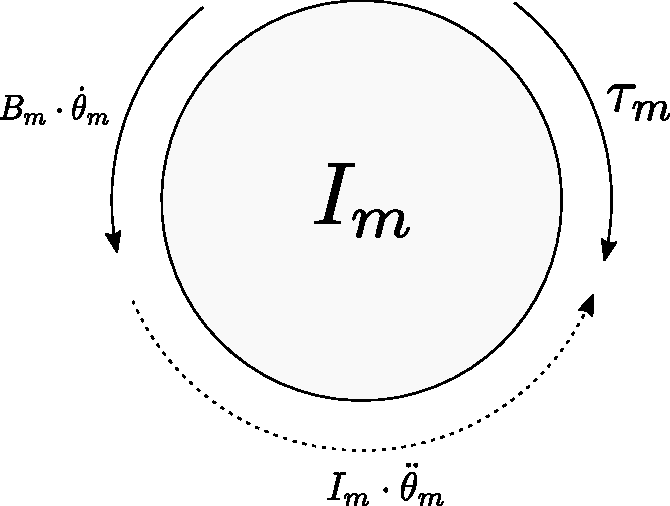
\includegraphics[scale=0.8]{figures/MotorMechanicalModel.pdf}
	\caption{A free body diagram of the motor}
	\label{fig:MotorMechanicalModel}
\end{figure}

From the figure an equation for the mechanical model can be derived.

\begin{flalign}\eq{
\tau_m(t)}{J_m \cdot \ddot{\theta}_m(t) + B \cdot \dot{\theta}_m(t)}
\end{flalign}

The equation is transferred into the frequency domain using the Laplace transform: 

\begin{flalign}\eq{
\tau(s)}{J_m(s) \cdot \omega_m \cdot s + B \cdot \omega_m}
\label{eq:ThetadotforBlock}
\end{flalign}

The mechanical model of the motor has be derived. The mechanical contributions from the motor will be used to model the drivetrain, in \secref{DriveTrain}. 

Next step is to model the electrical part of the motor, and to find the motors produced torque. 

\subsubsection{Electrical model}
The output needed from the motors electrical model is the torque, \si{\tau_m}. To obtain the torque, the formula for translating the electrical current, \si{i_a}, to torque is utilized:

\begin{flalign}\centering
  \si{\tau_m(t) = K_t \cdot i_a(t)} %\unit{\volt}
  \label{equ:motortorque}
\end{flalign}
\hspace{6mm} Where:\\
\begin{tabular}{p{1cm}ll}
& \si{\tau_m} & is the rotational force torque \unit{N \cdot m} \\
& \si{i_a(t)} & is the electrical closed loop current [A]\\
& \si{K_t} & is the torque constant [\si{\frac{N \cdot m}{A}}] \\
\end{tabular}

An expression for the current, \si{i_a}, is required to derive a model for the electrical system. In \figref{fig:electricaldiagrammotor} an electrical diagram of the motor is displayed.

\begin{figure}[H]
\centering
	\begin{circuitikz}[american voltages]
		\draw
		
		% electromotive force 
		(0,0) to [short] (6,0)
		%to [sV, l=$e_b$] (6,2) %  voltage
		(6,0) to [V, l=$e_b$] (6,3)
		%to node[short]{}(6,2)

		%to node[short]{}(0,0)		 
		(0,0) to [V, l=$V_m$] (0,3) %  voltage

		
		%to [R, l=$Z_G$] (3,3) % generator impedance
		
		(0,3) to [R, l_=$R_a$, i>_=$i_a$] (3,3)	
		
		to [L, l_=$L_a$] (6,3); 
	\end{circuitikz}
  \caption{A electrical diagram of the motor}
  \label{fig:electricaldiagrammotor}
\end{figure}

By using Kirchoffs voltage law on the closed loop, seen in \figref{fig:electricaldiagrammotor}, an expression including $i_a$ can be derived:

\begin{flalign}\eq{
V_m(t)}{R_a \cdot i_a(t) + L_a \cdot \frac{di_a}{dt} + e_b}\unit{V} 
\label{MotorClosedLoop}
\end{flalign}
\hspace{6mm} Where:\\
\begin{tabular}{p{1cm}ll}
& \si{V_m(t)} & is the supply voltage [V] \\
& \si{R_a} & is the internal resistance in the motor [$\Omega$]\\
& \si{L_a} & is the inductance in the motor [H] \\
& \si{e_b} & is the electromotive force, also called EMF [$\V$] \\
\end{tabular}

The electromotive force, \si{e_b}, is equivalent to:

\begin{flalign}\eq
{e_b}{K_e \cdot \dot{\theta}_m(t)}\unit{V} 
\end{flalign}
\hspace{6mm} Where:\\
\begin{tabular}{p{1cm}ll}
& \si{K_e} & is the electromotive constant [Wb] \\
& \si{\dot{\theta}_m} & is the angular velocity in the motor \unit{\frac{rad}{s}} \\
\end{tabular}

The equivalent for the electromotive force is substituted into \eqref{MotorClosedLoop}.

\begin{flalign}\eq{
V_m(t)}{R_a \cdot i_a(t) + L_a \cdot \frac{di_a}{dt} + K_e \cdot \dot{\theta}_m(t)}\unit{V}
\end{flalign}

The Laplace transform is applied to the derived equation:

\begin{flalign}
\eq{V_m(s)}{R_a \cdot i_a(s) + L_a \cdot s \cdot i_a(s) + K_e \cdot \omega_m(s)}\unit{V} 
\end{flalign}

The equation is solved for \si{i_a}:

\begin{flalign} \eq{
i_a(s)}{\frac{V_m(s) - K_e \cdot \omega_m(s)}{sL_a + R_a} }\unit{A}
\end{flalign}

By substituting the derived equation for $i_a$ into \eqref{equ:motortorque}, a new expression for the motors torque is derived. 

\begin{flalign}\eq{
  \tau_m}{K_t \cdot i_a(s) = K_t \cdot \frac{V_m(s) - K_e \cdot \omega_m(s)}{sL_a + R_a}} \unit{N\cdot m}
  \label{eq:Totaltorquewithcurrentexpression}
\end{flalign}

A equation for the electrical model relative to the motors torque has been derived.

\subsubsection{Block representation}

\eqref{eq:Totaltorquewithcurrentexpression} delivers the information needed to make a visual representation of the motor model. The input is the supply voltage, \si{V_m(s)} delivered to the motor and the output is the required torque, \si{\tau_m}, see \figref{fig:motormodelBlock}. The block representation of the system is used, when the system is to be simulated.

\begin{figure}[H]
	\centering
	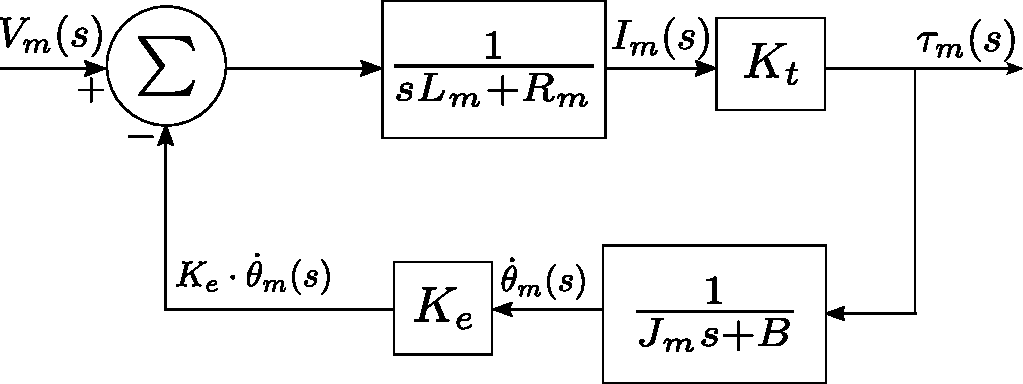
\includegraphics[scale=0.9]{figures/motormodelBlock.pdf}
	\caption{A block representation of the motor, with a voltage, \si{V_m(s)}, as the input and a rotational force, \si{\tau_m(s)}, as the output.}
	\label{fig:motormodelBlock}
\end{figure}

The angular velocity received from the drivetrain, see \figref{fig:Velocitymodelplantopen}, is dependent on the total inertia of the system, and is necessary to ensure the motor is affect by the load.

A model of the electrical and mechanical part has been formed and a block representation of the motors applied voltage and generated torque has been given. Next step is to model the drivetrain, which connects to the motor through the motor shaft.